\section{Data augmentation}
\label{sec:dataaugmentation}

This section describes both the data augmentation strategy for training and the cropping augmentation for inference.

\subsubsection{Data augmentation for Training}

Three data augmentation techniques are implemented to train the model.
The first two are commonly used in CV tasks, including random horizontal flips and traditional image adjustments like brightness, contrast, saturation, and hue variations.
For this, the standard ColorJitter method from PyTorch is used \cite{pytorch_colorJitter_docu}.
The third augmentation is the cropping mechanism, which reduces the image to the most relevant part.
Randomness is also introduced to enhance generalization.

\autoref{fig:tepNet_dataaugmentation} visualizes the cropping algorithm steps schematically.
At first, there are two green lines, which follow the train's ego-path and represent the \ac{GT} in the form of polylines.
Then the yellow rectangle is computed with this information, being the smallest possible rectangle around the \ac{GT}.
In the next step, the orange box, the start pixels of the rails \ac{GT} are centered by expanding the yellow borders in one direction.
Important to mention is that in this tailored dataset the rails always begin in the first row at the bottom of each image.
After that margins are added shown by the red rectangle.
These margins are predefined with hyperparameters.
After calculating the borders of the outermost box variability is added to enhance generalization and prevent biases.
The left, right, and top borders are moved by a distance calculated with a normal distribution, which is defined by hyperparameters.
This introduced variability follows the policy, which ensures that the starting pixels of the rails at the bottom stay in the cropped image.
\autoref{fig:tepNet_dataaugmentation} illustrates four augmented variations of the top image in the bottom row.

\begin{figure}[H]
    \centering
    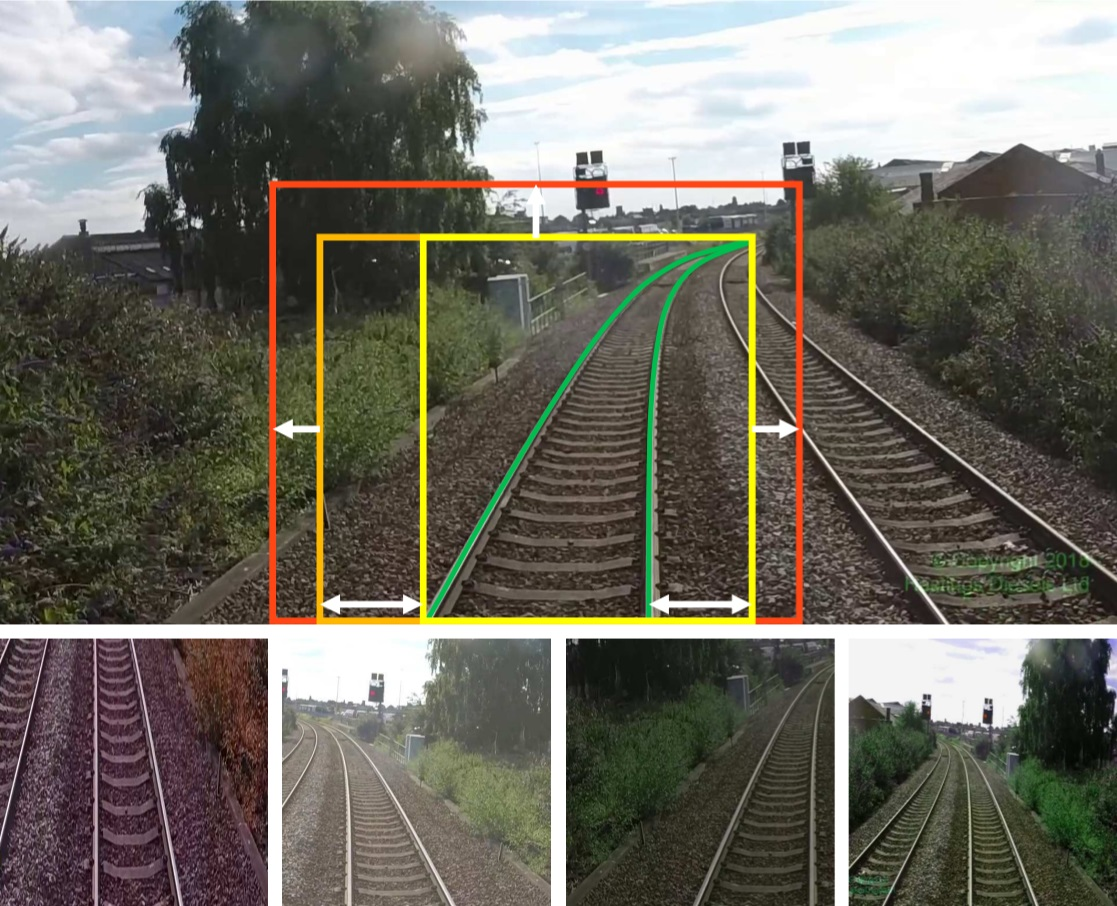
\includegraphics[width=0.6\linewidth]{PICs/Baselinepaper/data_augmenation.jpg}
    \caption{Data augmentation of \ac{TEP}-Net \cite{tepNet2024}, including the image horizontal flips, the color variations and the cropping mechanism.}
    \label{fig:tepNet_dataaugmentation}
\end{figure}

\subsubsection{Cropping in inference}

In \cite{tepNet2024} only cropped images are used for training the model to minimize the images to their most relevant \ac{ROI}.
For training and validating the model on the dataset, the \ac{GT} allows the computation of crop coordinates (left, top, right).
However, \ac{GT} data is unavailable in practical applications like video inference.
As a result, the crop coordinates must be, either predefined by a user or computed on the fly.

In a real-world application the ROI in the images changes, even when the camera is mounted in a fixed position.
Because of these perspective shifts when the train drives right or left turns, it easily can become unsustainable to have predetermined crop coordinates.
\autoref{fig:perspective_shifts} visualizes these perspective shifts.
The tighter the curve, the worse the shift.
The approach of \cite{tepNet2024} to solve this particular problem is the so-called "Autocrop".
This developed technique starts with the whole image, so the initial crop cords are the image borders.
After the initialization, the three coordinates (left, top, right) are updated according to the prediction of every new frame.
In more detail, new coordinates are calculated with a running average of the smallest rectangle around the prediction plus the predefined margins from the training.

\begin{figure}[H]
    \centering
    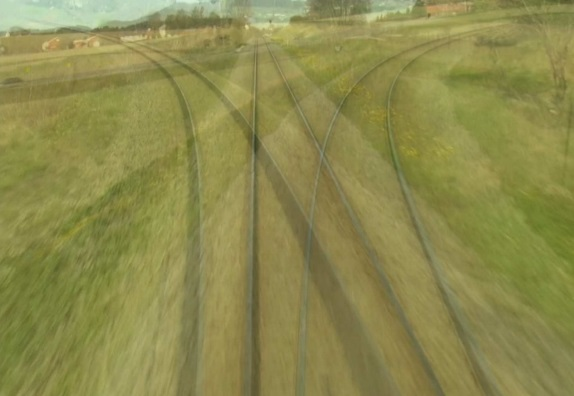
\includegraphics[width=0.6\linewidth]{PICs/Baselinepaper/perspective_shifts.jpg}
    \caption{Example of perspective shifts with three different scenarios: left curve, right curve and straight rail \cite{tepNet2024}.}
    \label{fig:perspective_shifts}
\end{figure}